\newpage
\section{Управление движением робота}
\begin{figure}[h]
    \centering
    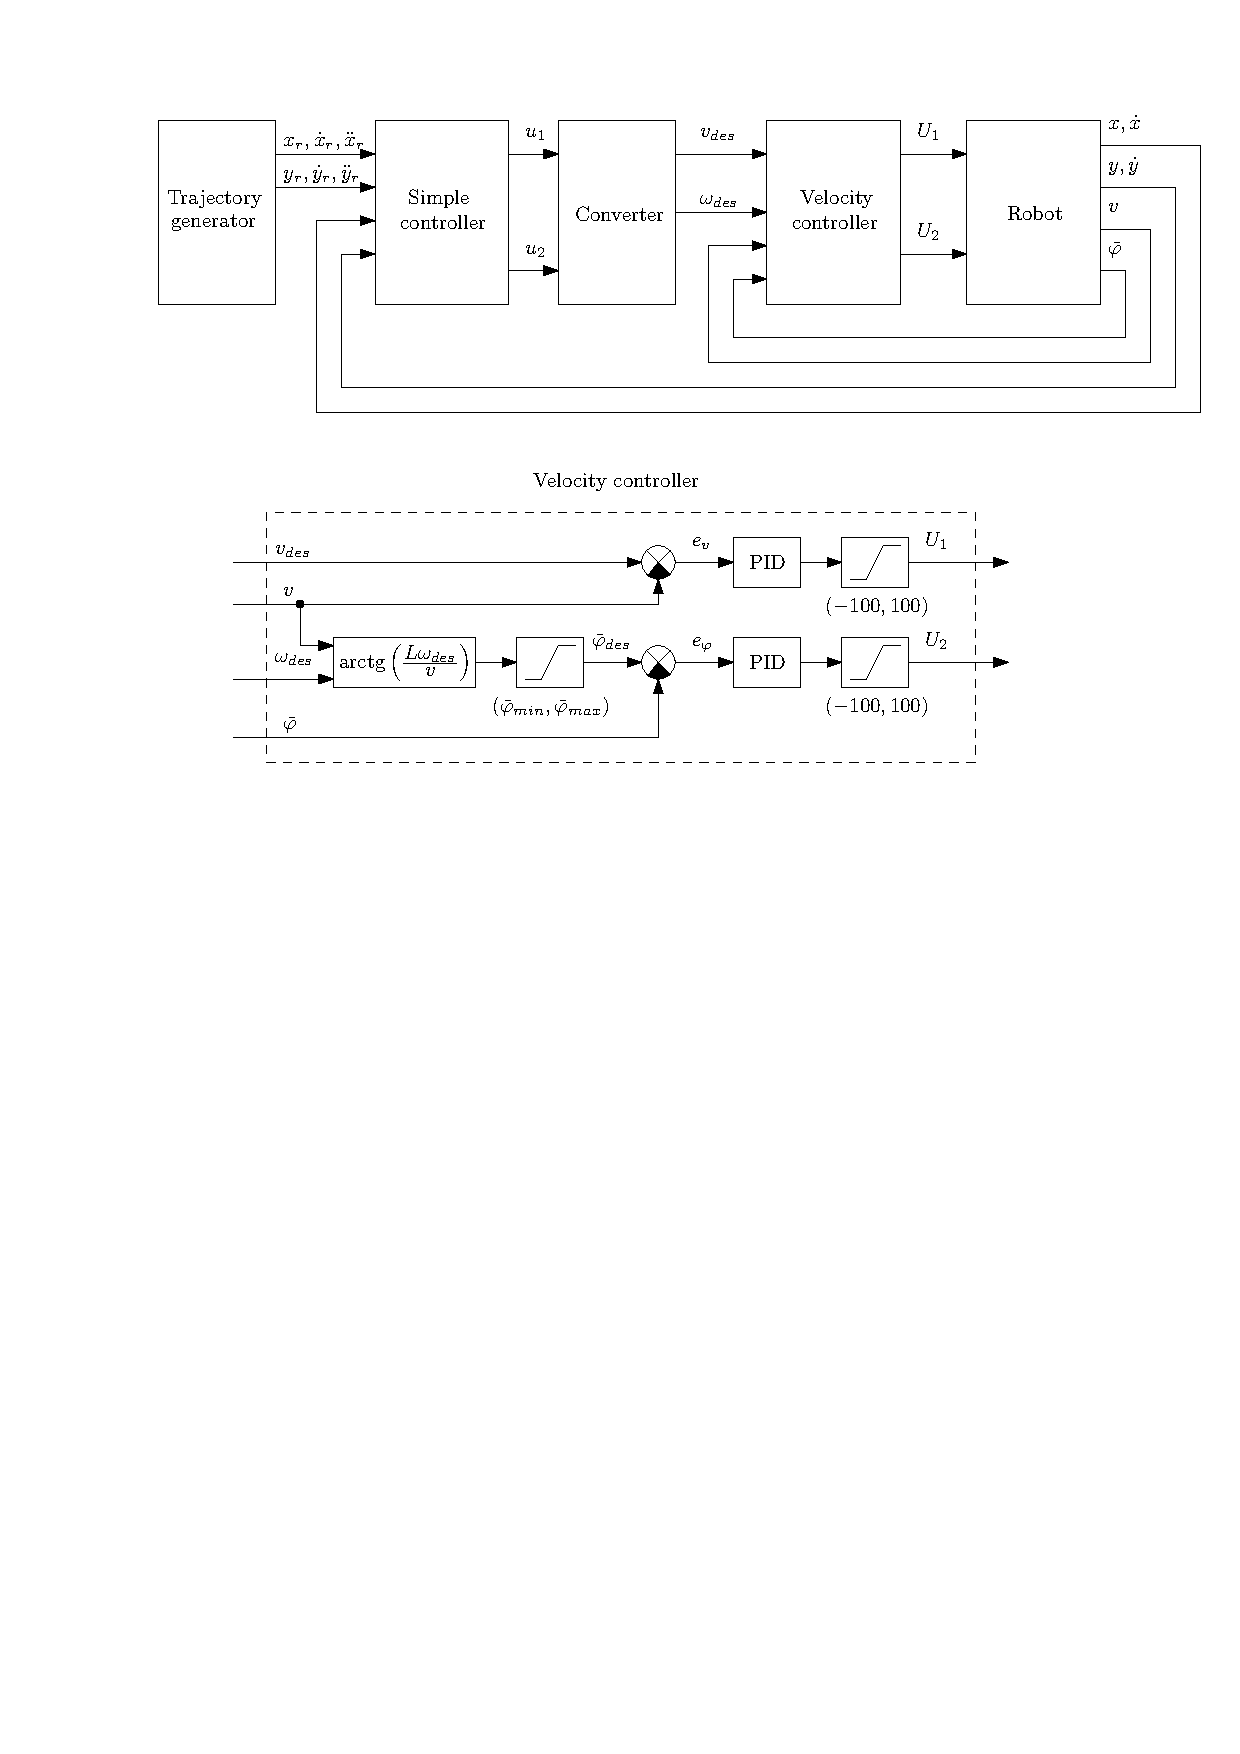
\includegraphics[width=\textwidth]{control_system.pdf}
    \caption{Структура системы управления движением робота.}
    \label{img_control_system}
\end{figure}
На рисунке~\ref{img_control_system}:\\
$U_1$~--- \% от максимального напряжения, подаваемого на двигатель, приводящий в движение задние колеса;\\
$U_2$~--- \% от максимального напряжения, подаваемого на рулевой двигатель;\\
$\bar\varphi$~--- угол поворота рулевого двигателя;\\
$v$ и $\omega$~--- текущие линейная и угловая скорости робота (последняя измеряется установленным на робота гироскопом);\\
$x$ и $y$~--- текущие координаты робота;\\
$x_r$ и $y_r$~--- координаты, которые должен иметь робот в данный момент времени, чтобы следовать по траектории;\\
$X_{des}$~--- желаемое значение величины~$X$;\\

Формулы для расчета некоторых из величин:
\begin{equation}
v = \omega_1 \cdot R,
\end{equation}
где $\omega_1$~--- скорость вращения тягового двигателя, $R$~--- радиус колес робота.

\begin{equation}
\bar{\varphi}_{min} = -\bar{\varphi}_{max}\ldotp
\end{equation}

Источник для~\eqref{firts}--\eqref{last}~--- это~\cite{de_luca}:
\begin{align}
& u_1 = \ddot{x}_r + k_{p1} (x_r - x) + k_{d1} (\dot{x}_r - \dot{x}) \label{firts}\\
& u_2 = \ddot{y}_r + k_{p2} (y_r - y) + k_{d2} (\dot{y}_r - \dot{y})
\end{align}

\begin{align}
& \dot{\xi} = u_1 \cos \theta + u_2 \sin \theta, \\
& v_{des} = \xi \\
& \omega_{des} = \frac{-u_1 \sin \theta + u_2 \cos \theta}{\xi} \label{last}
\end{align}

Кинематическая модель робота \cite{de_luca, survey}:
\begin{equation}
\left\{
\begin{aligned}
& \dot{x} = v \cos \theta \\
& \dot{y} = v \sin \theta \\
& \dot{\theta} = \frac{v}{L} \tan{\varphi}
\end{aligned}
\right.
\end{equation}
где $\varphi = L / r$, где в свою очередь $r$~--- радиус дуги, по которой движется робот; у мотоцикла и трицикла это угол поворота рулевого колеса.
